
\documentclass[showpacs,superscriptaddress,twocolumn,prl]{revtex4}
%%%%%%%%%%%%%%%%%%%%%%%%%%%%%%%%%%%%%%%%%%%%%%%%%%%%%%%%%%%%%%%%%%%%%%%%%%%%%%%%%%%%%%%%%%%%%%%%%%%%%%%%%%%%%%%%%%%%%%%%%%%%
\usepackage{amsmath}
\usepackage{amsfonts}
\usepackage{amssymb}
\usepackage{graphicx}

\setcounter{MaxMatrixCols}{10}
%TCIDATA{OutputFilter=LATEX.DLL}
%TCIDATA{Version=4.00.0.2312}
%TCIDATA{Created=Thursday, April 05, 2007 19:47:26}
%TCIDATA{LastRevised=Monday, April 21, 2008 00:18:44}
%TCIDATA{<META NAME="GraphicsSave" CONTENT="32">}
%TCIDATA{<META NAME="DocumentShell" CONTENT="Articles\SW\REVTeX 4">}
%TCIDATA{CSTFile=revtex4.cst}


\begin{document}

\title{Experimental demonstration of one-way quantum computation on an
ensemble quantum computer}
\author{First Author}
\affiliation{My Institution}
\author{Second Author}
\affiliation{My Institution}
\author{Third Author}
\affiliation{Other Institution}
\pacs{PACS number}
\pacs{PACS number}
\maketitle

\textbf{Being entirely different to the traditional quantum circuit model
\cite{Chuang} which is based on a network of unitary quantum logic gates,
the recently proposed one-way quantum computation model (one-way QC) \cite%
{onewayPRL,onewayPRA} invokes only a sequence of single-qubit measurements
to accomplish the computation, provided a highly entangled state - the
cluster state \cite{clusterstate} or some other special shaped graph states
\cite{othergraph} - is given in advance. This novel quantum computation
model has largely broadened people's view on quantum computation, and may
lead to a deep understanding on quantum entanglement and measurement.\ Here,
we report the first experimental investigation of the one-way QC in the
liquid-state NMR system by demonstrating a two-qubit Deutsch-Josza
algorithm. We show that due to the useage of the ensemble quantum
computation technology the active feed-forward in one-way QC is not
necessary. This is an import result for the future development of one-way
quantum computer.}

The quantum computer \cite{Chuang}, which utilize the laws of quantum
physics, is thought to be a powerful computation tool that can beat their
classical counterpart on some specific problems \cite{DJ,Grover,Shor}.
Though some pioneer works \cite{pioneer} have revealed its feasibility in a
primary step, it is still not very well understood that what are the
essential resources that give quantum computer this power. The one-way
quantum computation has opened up a possible way which will leads to a
further understanding on this important question. The entanglement and
measurement are particularly highlighted in this model, thus it is thought
that their role in quantum computation would be better understood by further
investigating into the one-way QC.

So far, Many works have been done which direct towards a better
understanding of the model \cite%
{othergraph,tworks,eworkn1,ework1,ework2,eworkn2,eworkdj}. These include a
few experiments which concentrate on the generation and characterization of
a few-qubit graph states upon linear optics \cite{eworkn1,ework1} and a
continuous variable system \cite{ework2}, the demonstration of one- and
two-qubit gates on a photonic 4-qubit linear cluster state \cite%
{eworkn1,eworkn2}, and the realization of a two-qubit search algorithm \cite%
{eworkn1,eworkn2} and a two-qubit Deutsch-Josza algorithm \cite{eworkdj}
both on the same photonic 4-qubit linear cluster state. Despite the exciting
progress these experimental works given, it is still far away to say that we
have understood this new quantum computation model very well. The one-way QC
is still an open field for both theoretical and practical research.

In this letter, we report the first experimental investigation of the
one-way QC in the liquid-state NMR system. We demonstrate a two-qubit
Deutsch-Josza algorithm on a star-like 4-qubit graph state (the first
one-way based realization of a quantum algorithm on a state other than the
4-qubit linear cluster state). The most remarkable feature which
distinguishes our experiment from the former works is the ensemble quantum
computing technology used here. As a consequence, we find no active
feed-forward (which is a crucial part in the one-way QC to guarantee the
determinacy and correctness of the computation) is needed in our experiment,
yet the computation is still deterministic and correct. This is entirely
different from all known experiments so far \cite{eworkn1,eworkn2,eworkdj}.
The technical challenges in realizing the active feed-forward are avoided by
this unique advantage. Thus this may be an import result for the future
development of one-way quantum computer.

Before the introduction to the experiment, we first give a brief review of
the Deutsch-Josza (DJ) algorithm \cite{DJ}. The DJ algorithm is a quantum
algorithm that can determine the global property of an unknown function with
fewer steps than classical methods. In this letter we consider the simplest
version of the DJ algorithm, which determines whether an unknown one-bit to
one-bit function $f$ is constant or balanced. There are four possible such
functions. Two of them, $f_{1}(x)=0$ and $f_{2}(x)=1$ ($x=0,1$), are defined
as constant functions, while the other two, $f_{3}(x)=x$ and $f_{4}(x)=\text{%
NOT }x$, are balanced functions. To classically accomplish this task one
needs to call the function twice to check both the outputs $f(0)$ and $f(1)$%
. But with DJ algorithm only one function call is needed. The process of the
algorithm is illustrated in Fig. \ref{djoracle}(a). Initially the two input
qubits, a target qubit and a control qubit (denoted by $t$ and $c$
respectively), are both prepared in the state $\left\vert +\right\rangle $ ($%
\left\vert +\right\rangle =\frac{1}{\sqrt{2}}(\left\vert 0\right\rangle
+\left\vert 1\right\rangle )$ is the eigenstate of the Pauli operator $%
\sigma _{x}$). Then they are inserted into an oracle which applies the
following unitary operations: first a $\sigma _{z}$ applied on the target
qubit, then the two-qubit operation $\left\vert x\right\rangle
_{c}\left\vert y\right\rangle _{t}\rightarrow \left\vert x\right\rangle
_{c}\left\vert y\oplus f_{j}(x)\right\rangle _{t}$ ($x,y\in \{0,1\}$)
corresponding to the specific funtion $f_{j}$ ($j=1,2,3,4$). The action of
the oracle is either preset or dictated by the outcome of another algorithm.
Finally the control qubit is measured by the operator $\sigma _{x}$. If the
outcome is $\left\vert +\right\rangle $ then the function is definitely to
be constant, otherwise it is balanced. Fig. \ref{djoracle}(b) shows all
possible oracles in terms of their quantum networks.

\begin{figure}[tbp]
\begin{center}
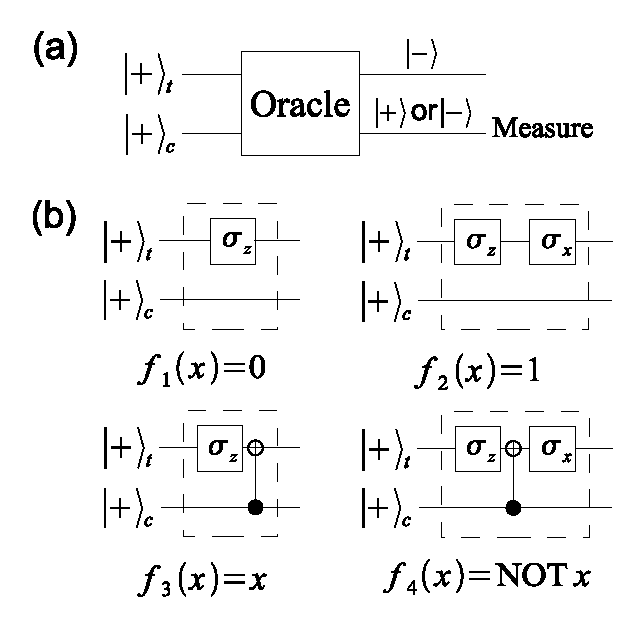
\includegraphics[ width=0.4\textwidth ]{fig1}
\end{center}
\caption{(a) Schematic illustration of the Deutsch-Josza algorithm. (b) The
quantum networks for all possible oracles. The inter-line symbol in the
network denotes the controlled-NOT gate $\left\vert 0\right\rangle
\left\langle 0\right\vert ^{(c)}\otimes \mathbb{I}^{(t)}+\left\vert
1\right\rangle \left\langle 1\right\vert ^{(c)}\otimes \protect\sigma %
_{x}^{(t)}$, where the superscripts denote the qubits and $\mathbb{I}$ is
identity.}
\label{djoracle}
\end{figure}

To implement the DJ algorithm one should be able to construct all the
possible four configurations. We find it is sufficient to do these on the
star-like 4-qubit graph state with appropriate single-qubit measurement
sequences and corresponding feed-forwards. In order to clearly describe how
we design the measurement sequences, we start with the introduction of the
general logical quantum circuit that can be realized on the star-like
4-qubit graph (Fig. \ref{graph}(a)), with arbitrary logical input states and
arbitrary single-qubit measurement bases in the $x$-$y$ plane. For this
purpose, as in Ref. \cite{onewayPRL}, we first prepare the four physical
qubits in the graph into the initial state $\left\vert \psi
_{t}\right\rangle _{1}\otimes \left\vert +\right\rangle _{2}\otimes
\left\vert +\right\rangle _{3}\otimes \left\vert \psi _{c}\right\rangle _{4}$%
, where the two arbitrary logical input states $\left\vert \psi
_{t}\right\rangle $ and $\left\vert \psi _{c}\right\rangle $ of the two
logical qubits \cite{logicqubit} (a target qubit and a control qubit) are
initially encoded on the physical qubits 1 and 4. Then all physical qubits
are entangled by the entangling operator%
\begin{equation}
S=S^{(12)}S^{(23)}S^{(42)},  \label{etangling}
\end{equation}%
where $S^{(jk)}=\left\vert 0\right\rangle \left\langle 0\right\vert
^{(j)}\otimes \sigma _{z}^{(k)}+\left\vert 1\right\rangle \left\langle
1\right\vert ^{(j)}\otimes \mathbb{I}^{(k)}$ is a controlled-phase gate
applied on the physical qubits $j$ and $k$ \cite{cphase}. The logical
information is now delocalized. It is then manipulated by the measurements
carried on the physical qubits 1 and 2 with the bases $B_{1}(\alpha
_{1})=\{\left\vert \alpha _{1+}\right\rangle _{1},\left\vert \alpha
_{1-}\right\rangle _{1}\}$ and $B_{2}(\alpha _{2})=\{\left\vert \alpha
_{2+}\right\rangle _{2},\left\vert \alpha _{2-}\right\rangle _{2}\}$
respectively, where $\left\vert \alpha _{\pm }\right\rangle =\frac{1}{\sqrt{2%
}}(\left\vert 0\right\rangle \pm e^{i\alpha }\left\vert 1\right\rangle )$
and $\alpha _{1},\alpha _{2}$ are arbitrary angles. After the measurements
the logical target qubit is transferred to the physical qubit 3, while the
logical control qubit is still encoded on the physical qubit 4. The
effective logical quantum circuit performed on the two logical qubits for
the above process is shown in Fig. \ref{graph}(b). The $s_{1}$ and $s_{2}$
in the circuit denote the outcome of the two measurements, where $s_{j}=0(1)$
corresponds to the state $\left\vert \alpha _{j+}\right\rangle (\left\vert
\alpha _{j-}\right\rangle )$ ($j=1,2$). The presence of the $s_{1}$ and $%
s_{2}$ represents the randomness introduced by the single-qubit
measurements, which may make the computation nondeterministic. This can be
overcome in the one-way QC by adopting appropriate feed-forward, which means
adjusting the future measurement basis according to the outcome of the
preceding measurements \cite{onewayPRL}.

\begin{figure}[tbp]
\begin{center}
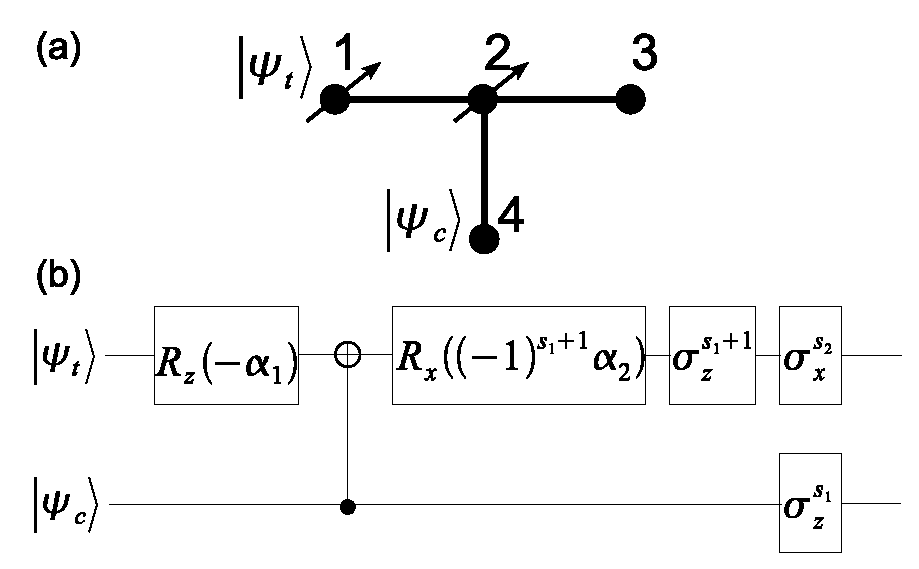
\includegraphics[ width=0.45\textwidth ]{fig2}
\end{center}
\caption{(a) The star-like 4-qubit graph. The vertices represent the four
physical qubits, and each edge between them indicates a controlled-phase
gate applied on the connected qubits when to produce the entangled state.
The arrows marked on vertices 1 and 2 denote the measurements. For the
detailed description of the initial state, entangling, and measurements, see
the text. (b) The general logical quantum circuit realized on the above
graph with arbitrary logical input states and arbitrary measurement bases. $%
R_{n}(\protect\alpha )=e^{-i\protect\alpha \protect\sigma _{n}/2}$ $(n=x,z)$%
. }
\label{graph}
\end{figure}

The design of the resource entangled state and the single-qubit measurement
sequences for implementing the DJ algorithm is done by comparing the general
logical circuit in Fig. \ref{graph}(b) with the networks in Fig. \ref%
{djoracle}(b). Since the input state in the DJ algorithm is $\left\vert
+\right\rangle \otimes \left\vert +\right\rangle $, we set $\left\vert \psi
_{t}\right\rangle =\left\vert \psi _{c}\right\rangle =\left\vert
+\right\rangle $. The resulted entangled state, $\left\vert \psi _{\text{G}%
}\right\rangle =\left\vert +\right\rangle _{1}\left\vert 0\right\rangle
_{2}\left\vert -\right\rangle _{3}\left\vert +\right\rangle _{4}+\left\vert
-\right\rangle _{1}\left\vert 1\right\rangle _{2}\left\vert +\right\rangle
_{3}\left\vert -\right\rangle _{4}$, which is produced by performing the
entangling operator $S$ on the initial state $\left\vert +\right\rangle
_{1}\otimes \left\vert +\right\rangle _{2}\otimes \left\vert +\right\rangle
_{3}\otimes \left\vert +\right\rangle _{4}$, is exactly the 4-qubit graph
state which corresponds to the star-like 4-qubit graph \cite{onewayPRA} (it
is also equivalent to the 4-qubit GHZ state under local unitary operations).
The measurement bases and the corresponding feed-forward operations which
are chosen to reproduce the networks of all possible oracles are summarized
in the Table \ref{table}. Note in the design of the measurements which
correspond to the constant functions $f_{1}$ and $f_{2}$, the fact is used
that a CNOT gate is equivalent to the identity operation when it acts on the
state $\left\vert +\right\rangle \otimes \left\vert +\right\rangle $. The
final result of the algorithm is read by measuring the physical qubit 4. If
its state (after accounting for the feed-forward operation) is $\left\vert
+\right\rangle (\left\vert -\right\rangle )$ then the function is
constant(blanced).

\begin{table}[tb]
\caption{Measurement bases and feed-forward operations for implementing the
DJ algorithm. $\text{FF}^{(3)}$ and $\text{FF}^{(4)}$ represent the
feed-forward operations on physical qubits 3 and 4. They can be accounted
for by adjusting the measurement basis of the final read-out.}
\label{table}%\begin{center}
\begin{tabular*}{0.48\textwidth}{@{\extracolsep{\fill}}cccc}
\hline\hline
& Measurement bases & $\text{FF}^{(3)}$ & $\text{FF}^{(4)}$ \\ \hline
$f_{1}$ & $B_{1}(0),B_{2}(0)$ & $\sigma_{z}^{s_{1}}\sigma_{x}^{s_{2}+1}$ & $%
\sigma_{z}^{s_{1}}$ \\
$f_{2}$ & $B_{1}(0),B_{2}(0)$ & $\sigma_{z}^{s_{1}}\sigma_{x}^{s_{2}}$ & $%
\sigma_{z}^{s_{1}}$ \\
$f_{3}$ & $B_{1}(\pi),B_{2}(0)$ & $\sigma_{z}^{s_{1}+1}\sigma_{x}^{s_{2}}$ &
$\sigma_{z}^{s_{1}}$ \\
$f_{4}$ & $B_{1}(\pi),B_{2}(0)$ & $\sigma_{z}^{s_{1}+1}\sigma_{x}^{s_{2}+1}$
& $\sigma_{z}^{s_{1}}$ \\ \hline\hline
\end{tabular*}
%\end{center}
\end{table}

In the experiment we use the spins of the four $^{13}$C nuclei in the
crotonic acid (Fig. \ref{crotacid}) as the four physical qubits. The sample
was dissolved in $\text{D}_{2}\text{O}$. The reduced hamiltonian for the
four $^{13}$C nuclei is written as $H_{0}=\sum_{j=1}^{4}\omega
_{j}I_{z}^{(j)}+2\pi \sum_{j<k}^{4}J_{jk}I_{z}^{(j)}I_{z}^{(k)}$ with the
Larmor angular frequencies $\omega _{j}$ and $J$-coupling strengths $J_{jk}$%
. The values of these parameters are listed in Fig. \ref{crotacid}.

\begin{figure}[tbp]
\begin{center}
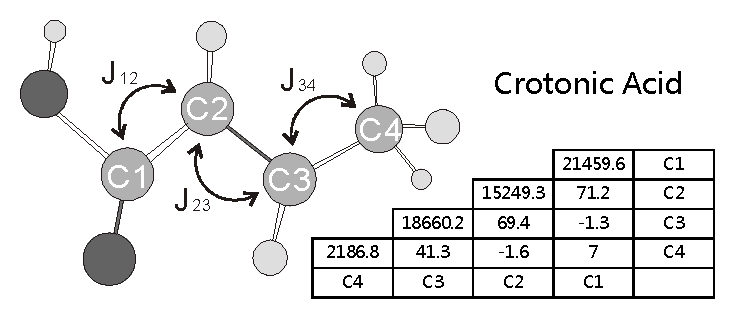
\includegraphics[ width=0.45\textwidth ]{fig3}
\end{center}
\caption{Molecular structure of crotonic acid with a table of the chemical
shifts (on the diagonal) and $J$-coupling constants (below the diagonal).
The parameters are given in unit Hz.}
\label{crotacid}
\end{figure}

%\begin{table}[tb]
%\caption{NMR parameters for crotonic acid.}
%\label{table2}%\begin{center}
%\begin{tabular*}{0.48\textwidth}{@{\extracolsep{\fill}}cccccc}
%\hline\hline
%& $\nu $/Hz & $J _{\text{C}_{1}}$/Hz & $J _{\text{C}_{2}}$/Hz & $J _{\text{C}%
%_{3}}$/Hz & $J _{\text{C}_{4}}$/Hz \\ \hline
%$\text{C}_{1}$ & 21459.6 &  & 71.2 & -1.3 & 7 \\
%$\text{C}_{2}$ & 15249.3 & 71.2 &  & 69.4 & -1.6 \\
%$\text{C}_{3}$ & 18660.2 & -1.3 & 69.4 &  & 41.3 \\
%$\text{C}_{4}$ & 2186.8 & 7 & -1.6 & 41.3 &  \\ \hline\hline
%\end{tabular*}
%%\end{center}
%\end{table}

The experimental generation of the 4-qubit graph state is divided into three
steps. Firstly, preparing the pseudopure state $\left\vert 0000\right\rangle
$ of the four $^{13}$C nuclear spins from the thermal equilibrium deviation
density matrix $\sum\nolimits_{j=1}^{4}\sigma _{z}^{(j)}$. Secondly,
preparing the 4-qubit GHZ state $\left\vert 0\right\rangle ^{\otimes
4}+\left\vert 1\right\rangle ^{\otimes 4}$ from $\left\vert
0000\right\rangle $ by the unitary operation $U_{\text{GHZ}}=\text{CNOT}%
^{(34)}\text{CNOT}^{(23)}\text{CNOT}^{(12)}\text{H}^{(1)}$, where $\text{H}=%
\frac{1}{\sqrt{2}}(\sigma _{x}+\sigma _{z})$ is the Hadamard gate. The $%
\text{CNOT}^{(jk)}$ could be further decomposed into (in time-reversed order)%
\begin{equation}
R_{y}^{(k)}(\frac{\pi }{2})-e^{-i\frac{\pi }{4}\sigma _{z}^{(j)}\sigma
_{z}^{(k)}}-R_{-x}^{(k)}(\frac{\pi }{2})-R_{-z}^{(j)}(\frac{\pi }{2}%
)-R_{-z}^{(k)}(\frac{\pi }{2}),
\end{equation}%
where $R_{y}^{(k)}(\frac{\pi }{2})=e^{-i(\pi /2)\sigma _{y}^{(k)}/2}$
denotes a $\frac{\pi }{2}$-rotation of the qubit $k$ around the $\hat{y}$
axis, and so forth. The $J$-coupling gate $e^{-i\frac{\pi }{4}\sigma
_{z}^{(j)}\sigma _{z}^{(k)}}$ can be realized by the free evolution of the
spin system under $H_{0}$ with appropriate refocusing operations. Those $%
\hat{z}$ rotations in CNOT gates can be moved to the beginning of $U_{\text{%
GHZ}}$ by appropriate transformation skills \cite{nmrreview}, where they are
safely annihilated since $\hat{z}$ rotations take no effect on the state $%
\left\vert 0000\right\rangle $. Hence the sequence of the operations is
largely simplified.\ Finally, the 4-qubit graph state $\left\vert \psi _{%
\text{G}}\right\rangle $ is generated from the GHZ state by the local
unitary operations $\text{H}^{(1)}R_{-y}^{(3)}(\frac{\pi }{2})\text{H}^{(4)}$%
.

The required single-qubit projective measurements in the one-way QC are
absent in current NMR quantum computing technologies. But instead we can use
the pulsed magnetic field gradients to mimic them \cite{measure}, whose
effect is equivalent to that by applying these projective measurements on
every member of the ensemble. For example, one could use the operations (in
time-reversed order)%
\begin{gather}
P_{z}^{(1)}=R_{-y}^{(4)}(\pi )-R_{-y}^{(3)}(\pi )-G_{1}-R_{-y}^{(4)}(\pi
)-R_{-y}^{(2)}(\pi )-G_{1}  \notag \\
-R_{y}^{(4)}(\pi )-R_{y}^{(3)}(\pi )-G_{1}-R_{y}^{(4)}(\pi )-R_{y}^{(2)}(\pi
)-G_{1}
\end{gather}%
to mimic the $\sigma _{z}^{(1)}$ measurement on the physical qubit 1, where $%
G_{1}$ is the pulsed magnetic field gradient along $\hat{z}$ with a period
of $\tau _{1}/4$. These operations dephase all the coherences which are
associated with the transitions of qubit 1 in the density matrix $\rho
=\left\vert \Phi \right\rangle \left\langle \Phi \right\vert $ (suppose $%
\left\vert \Phi \right\rangle =\left\vert 0\right\rangle _{1}\left\vert \phi
_{0}\right\rangle +\left\vert 1\right\rangle _{1}\left\vert \phi
_{1}\right\rangle $, where $\left\vert \phi _{0(1)}\right\rangle $ is the
state of the other three qubits), resulting an ensemble-average density
matrix $\left\vert 0\right\rangle _{1}\left\langle 0\right\vert \left\vert
\phi _{0}\right\rangle \left\langle \phi _{0}\right\vert +\left\vert
1\right\rangle _{1}\left\langle 1\right\vert \left\vert \phi
_{1}\right\rangle \left\langle \phi _{1}\right\vert $, which is exactly the
same as the result by performing projective measurement $\sigma _{z}^{(1)}$
on every member of the ensemble. To mimic the measurement $\sigma _{x}^{(1)}$
one just first rotate the qubit 1 to the $\hat{z}$ axis before $P_{z}^{(1)}$%
. In our experiment we use the sequences $P_{z}^{(1)}-R_{-y}^{(1)}(\frac{\pi
}{2})$ and $P_{z}^{(1)}-R_{y}^{(1)}(\frac{\pi }{2})$ to mimic the
measurements with the bases $B_{1}(0)$ and $B_{1}(\pi )$ respectively. We
left the qubit 1 along $\hat{z}$ after the "measurement" for the purpose
that its state could label the "measurement" outcome, i.e., $\left\vert
0\right\rangle _{1}\left\langle 0\right\vert $ denotes $s_{1}=0$ and $%
\left\vert 1\right\rangle _{1}\left\langle 1\right\vert $ denotes $s_{1}=1$.
The measurement on qubit 2 with basis $B_{1}(0)$ is mimicked by a similar
sequence $P_{z}^{(2)}-R_{-y}^{(2)}(\frac{\pi }{2})$, where%
\begin{gather}
P_{z}^{(2)}=G_{2}-R_{-y}^{(4)}(\pi )-R_{-y}^{(1)}(\pi
)-G_{2}-R_{-y}^{(4)}(\pi )-R_{-y}^{(3)}(\pi )  \notag \\
-G_{2}-R_{y}^{(4)}(\pi )-R_{y}^{(1)}(\pi )-G_{2}-R_{y}^{(4)}(\pi
)-R_{y}^{(3)}(\pi ),
\end{gather}%
$G_{2}$ is the pulsed magnetic field gradient with a period of $\tau _{2}/4$
($\tau _{2}\neq \tau _{1}$).

The randomness associated with projective measurements is avoided by the
effective ensemble measurements above. As a consequence, the active
feed-forward (i.e., the real-time adjusting of the measurement basis
according to the outcome of the preceding measurements during the
computation) is not required in our experiment, yet the computation is still
deterministic. Since all measurement outcome is recorded in the resulting
mixed state, one could choose a sequence of the measurement outcome in
advance to denote in which subspace the computation is actually taken place.
Hence all measurement bases can be determined priorly, including all
necessary feed-forward. In our experiment we choose this computational
subspace as $s_{1}=s_{2}=0$. Consequently, in this subspace no feed-forward
needs to be accounted for at the read-out stage, since the feed-forward
operation $\sigma _{z}^{s_{1}}$ on the qubit 4 - the read-out particle - is
reduced to identity. (The feed-forward operation on qubit 3 is ignored since
it is not the read-out qubit.)

The experiment was implemented on a Bruker UltraShield 500 spectrometer at
room temperature. In the practical implementation, all the single-qubit
operations above are realized by sequences of strongly modulating NMR pulses
\cite{smp}. We maximize the gate fidelity of the simulated propagator to the
ideal gate, and we also maximize the effective gate fidelity by averaging
over a weighted distribution of radio frequency (RF) Field strengths,
because the RF-control fields are inhomogeneous over the sample, although
it's hard to fully overcome. Theoretically the gate fidelities we calculated
for every pulse are greater than 0.99, and the pulse lengths range from 300
to 700 $\mu s$.

A full state tomography was performed to the obtained graph state $\rho _{%
\text{exp}}$ (Fig. \ref{exgraphstate}), yielding the fidelity $%
F=\left\langle \psi _{\text{G}}\right\vert \rho _{\text{exp}}\left\vert \psi
_{\text{G}}\right\rangle =0.74$. By exploiting the entanglement witness \cite%
{witness} $W=I/2-\left\vert \psi _{\text{G}}\right\rangle \left\langle \psi
_{\text{G}}\right\vert $ ($I$ denotes identity operatior), one can easily
prove the presence of genuine four-partite entanglement here, since a
negative expectation value of $W$ is obtained (Tr$(W\rho _{\text{exp}})=-0.24
$). Fig. \ref{finalresult} shows the diagonal elements of the final density
matrices of the four particles at the end of the algorithm. The off-diagonal
elements were not measured since they are irrelevant to the final readout
and are all $0$s in theory. Remember the computation is taken place in the
subspace $s_{1}=s_{2}=0$, thus the algorithm result should be read in the
corresponding subspace where particle 1 and 2 are in state $\left\vert
00\right\rangle $. The substantial loss in signal intensity arises from
decoherence, B1 inhomogeneity effects and imperfect pluses. It shows the
fidelity of the network is about 74\%, smaller than the expected over 95\%
for an ideal implementation. Our calculations indicate that in the absence
of incoherent effects an overall fidelity of about 85\% could be achieved.
Nevertheless, our experiment result still shows a good performance of the
algorithm when compared with the theoretical expectation.

\begin{figure}[tbp]
\begin{center}
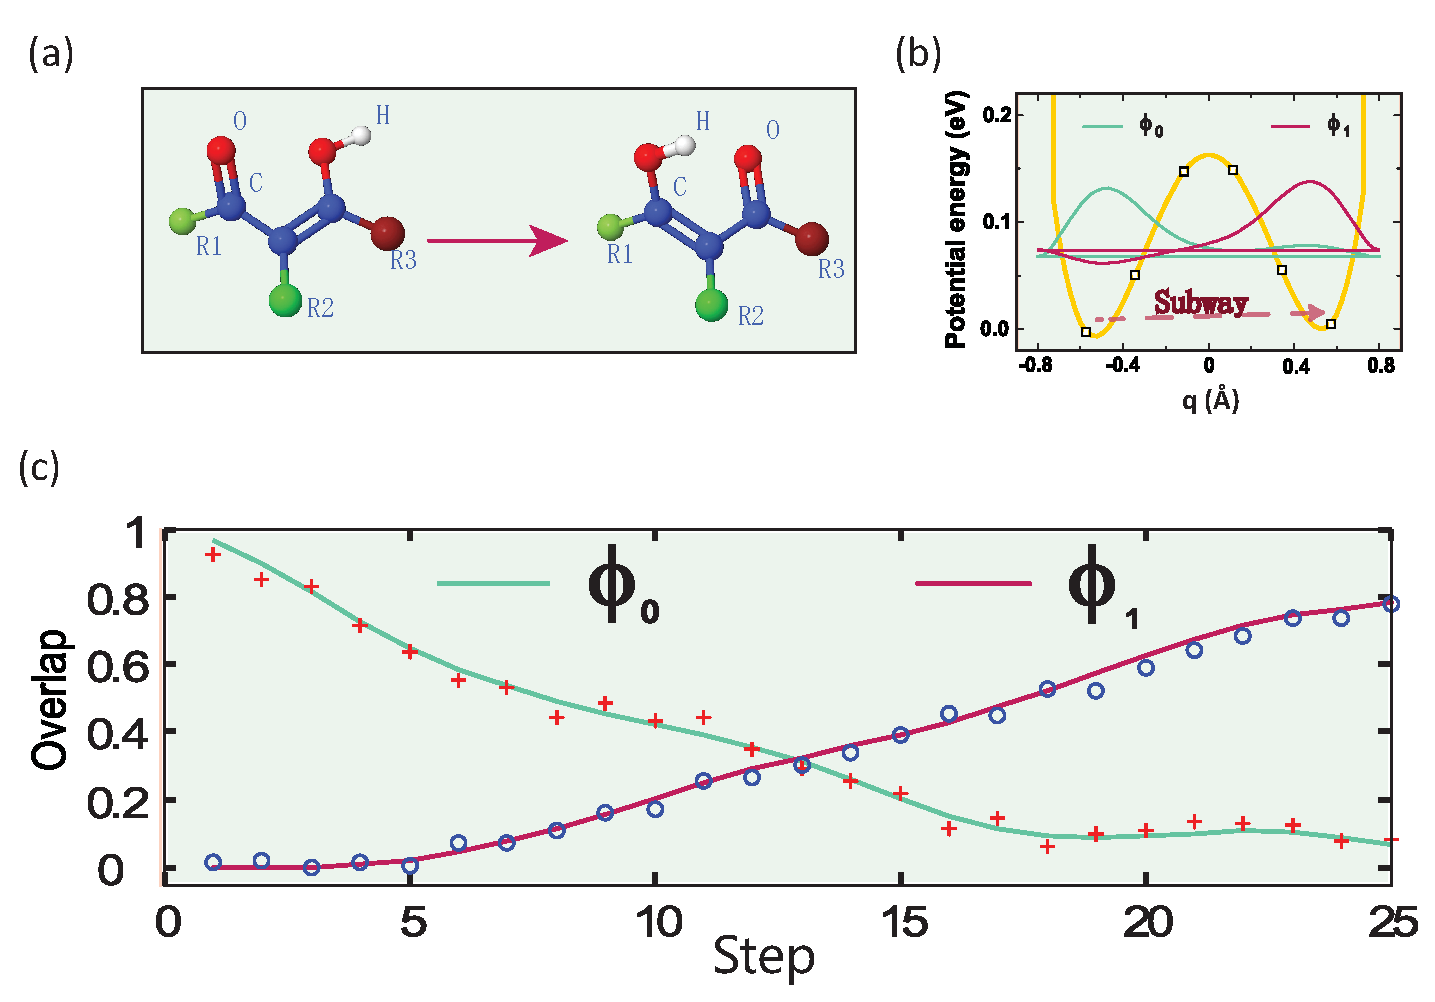
\includegraphics[ width=0.45\textwidth ]{fig4}
\end{center}
\caption{(color online). The ideal (a) and measured (b) density matrices of
the star-like four-qubit graph state $\left\vert +0-+ \right\rangle +
\left\vert -1+- \right\rangle $.}
\label{exgraphstate}
\end{figure}

\begin{figure}[tbp]
\begin{center}
\includegraphics[ width=0.45\textwidth ]{fig5}
\end{center}
\caption{(color online). The measured (color bars) and ideal (dashed bars)
diagonal elements of the final density matrices of the four particles. The
state of particle 4 in subspace $\left\vert 0\right\rangle _1 \left\vert
0\right\rangle _2$ represents the algorithm result.}
\label{finalresult}
\end{figure}

In conclusion, we have designed and demonstrated an one-way based
realization of the DJ algorithm on a star-like four-qubit graph state. This
is the first one-way experiment reported which is performed in the
liquid-state NMR system and on a state other than the linear four-qubit
cluster state. Due to the ensemble quantum computing technology used here,
we find no active feed-forward is needed in our experiment yet the
computation is still deterministic and correct. This unique and interesting
feature avoids the technical challenges in realizing the active
feed-forward. Our experimental results are in good agreement with the
theoretical expectation.

\begin{thebibliography}{99}
\bibitem{Chuang} M. A. Nielsen and I. L. Chuang, \textit{Quantum Computing
and Quantum Information} (Cambridge University Press, Cambridge, England,
2000).

\bibitem{onewayPRL} R. Raussendorf and H. J. Briegel, Phys. Rev. Lett.
\textbf{86}, 5188 (2001).

\bibitem{onewayPRA} R. Raussendorf, D. E. Browne, and H. J. Briegel, Phys.
Rev. A \textbf{68}, 022312 (2003).

\bibitem{clusterstate} H. J. Briegel and R. Raussendorf, Phys. Rev. Lett.
\textbf{86}, 910 (2001).

\bibitem{othergraph} M. Van den Nest, A. Miyake, W. D\"{u}r, and H. J.
Briegel, Phys. Rev. Lett. \textbf{97}, 150504 (2006).

\bibitem{DJ} D. Deutsch and R. Jozsa, Proc. R. Soc. London A, \textbf{439},
553 (1992).

\bibitem{Shor} P. W. Shor, SIAM J. Sci. Stat. Comput. \textbf{26}, 1484
(1997).

\bibitem{Grover} L. K. Grover, Phys. Rev. Lett. \textbf{79}, 325 (1997).

\bibitem{pioneer} I. L. Chuang, L. M. K. Vandersypen, X. Zhou, D. W. Leung,
and S. Lloyd, Nature \textbf{393}, 143 (1998); J. A. Jones, M. Mosca, and R.
H. Hansen, Nature \textbf{393}, 344 (1998); L. M. K. Vandersypen \textit{et
al.}, Nature \textbf{414}, 883 (2001).

\bibitem{tworks} M. A. Nielsen, Phys. Rev. Lett. \textbf{93}, 040503 (2004);
M. S. Tame, M. Paternostro, M. S. Kim, and V. Vedral, Phys. Rev. A \textbf{72%
}, 012319 (2005); N. Yoran and A. J. Short, Phys. Rev. Lett. \textbf{96},
170503 (2006); D. Gross, K. Kieling, and J. Eisert, Phys. Rev. A \textbf{74}%
, 042343 (2006); V. Danos and E. Kashefi, Phys. Rev. A \textbf{74}, 052310
(2006).

\bibitem{eworkn1} P. Walther \textit{et al.}, Nature \textbf{434}, 169
(2005).

\bibitem{ework1} P. Walther, M. Aspelmeyer, K. J. Resch, and A. Zeilinger,
Phys. Rev. Lett. \textbf{95}, 020403 (2005); N. Kiesel \textit{et al.},
Phys. Rev. Lett. \textbf{95}, 210502 (2005); A.-N. Zhang \textit{et al.},
Phys. Rev. A \textbf{73}, 022330 (2006); C.-Y. Lu \textit{et al.}, Nature
Phys. \textbf{3}, 91 (2007).

\bibitem{ework2} X. Su \textit{et al.}, Phys. Rev. Lett. \textbf{98}, 070502
(2007).

\bibitem{eworkn2} R. Prevedel \textit{et al.}, Nature \textbf{445}, 65
(2007).

\bibitem{eworkdj} M. S. Tame \textit{et al.}, Phys. Rev. Lett. \textbf{98},
140501 (2007).

\bibitem{logicqubit} A detailed introduction of the logical qubits and
physical qubits can be found in \cite{eworkn1}.

\bibitem{cphase} Note that some papers use another controlled-phase gate $%
S=\left\vert 0\right\rangle \left\langle 0\right\vert \otimes \mathbb{I}%
+\left\vert 1\right\rangle \left\langle 1\right\vert \otimes \sigma _{z}$ as
the entangling operator. The produced graph states with these two entangling
operators are equivalent up to local unitary operations.

\bibitem{nmrreview} L. M. K. Vandersypen and I. L. Chuang, Rev. Mod. Phys.
\textbf{76}, 1037 (2005).

\bibitem{measure} G. Teklemariam, E. M. Fortunato, M. A. Pravia, T. F.
Havel, and D. G. Cory, Phys. Rev. Lett. \textbf{86}, 5845 (2001).

\bibitem{smp} E. M. Fortunato \textit{et al.}, J. Chem. Phys. \textbf{116},
7599 (2002).

\bibitem{witness} G. T\'{o}th and O. G\"{u}hne, Phys. Rev. A \textbf{72},
022340 (2005).
\end{thebibliography}

\end{document}
